% Index of /design/

\section{Mockups}
\label{sec:Mockups}

\begin{wrapfigure}[8]{r}{6cm}
	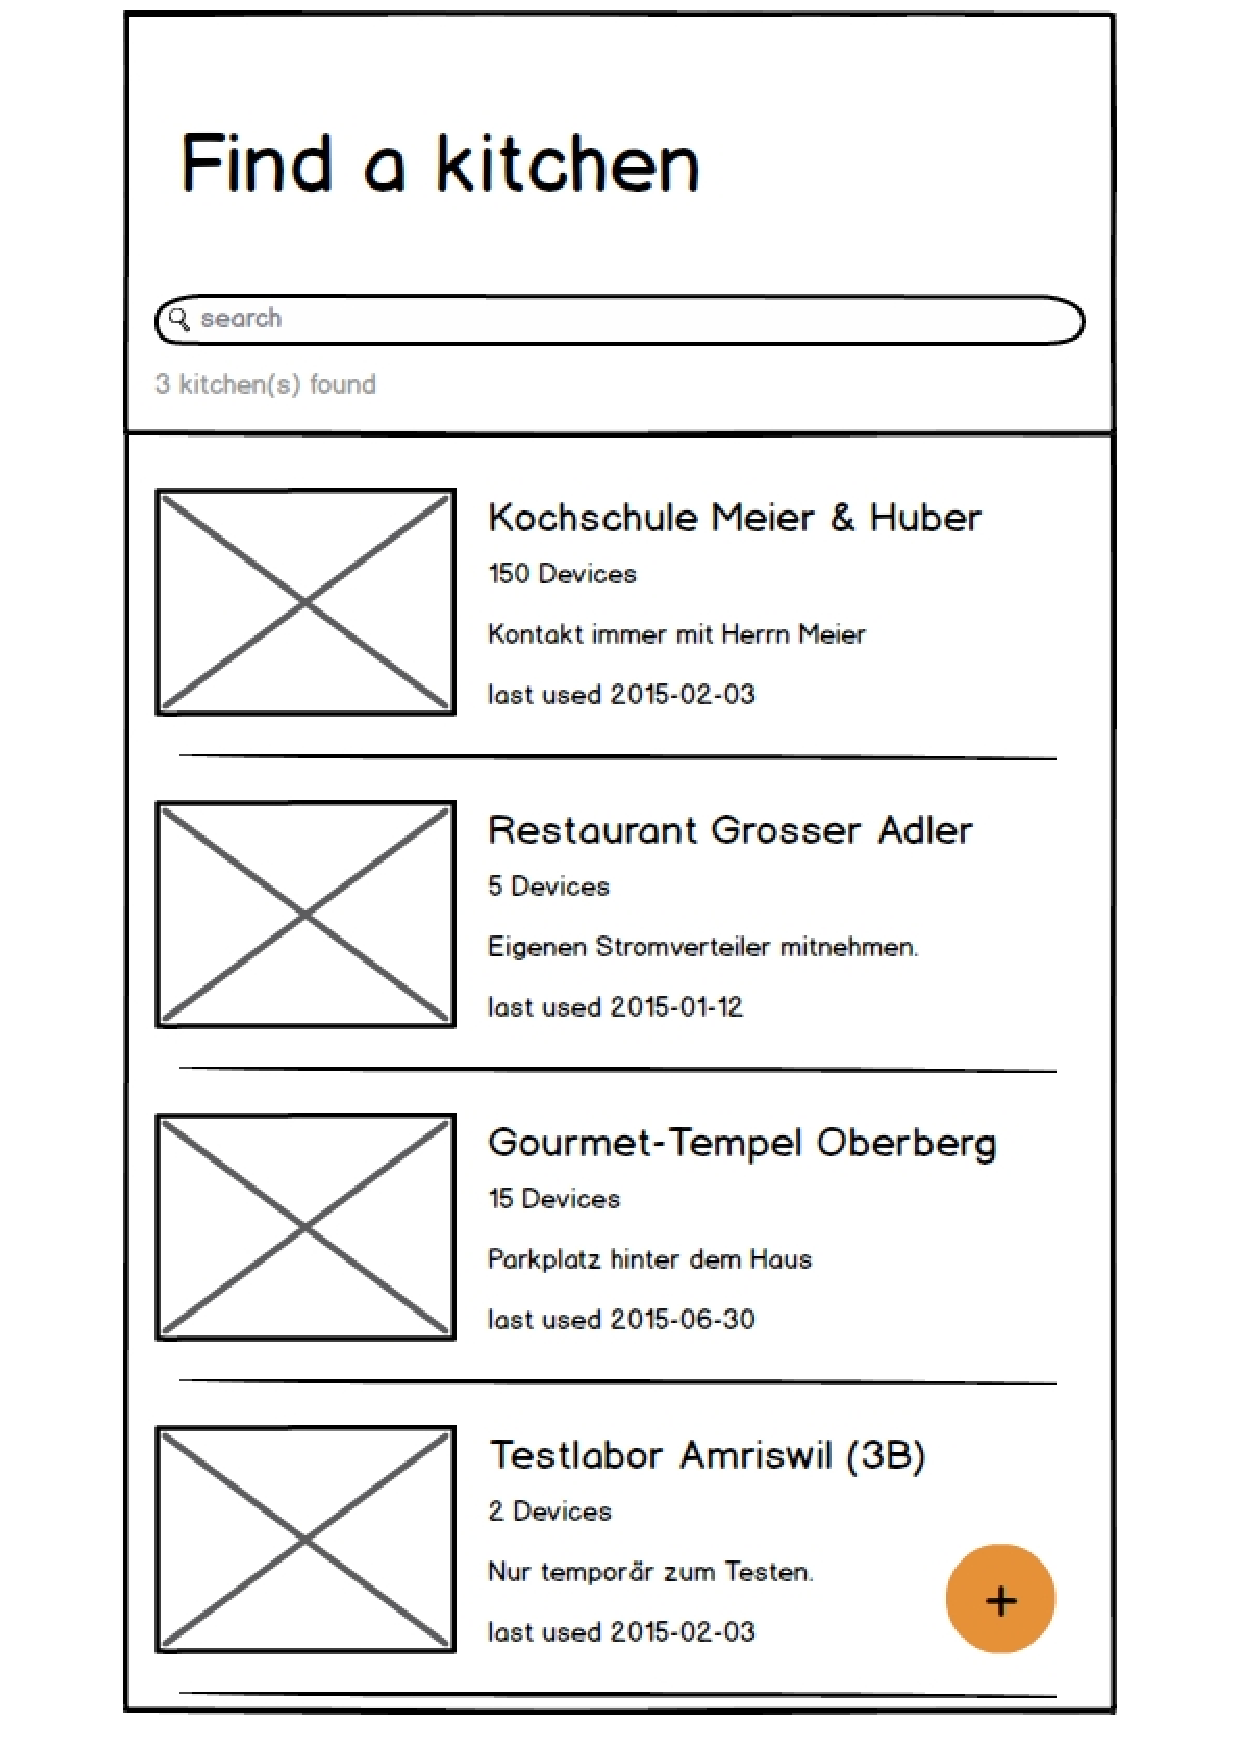
\includegraphics[page=1,trim=0 0 0 0,clip,scale=0.21]{uiux/res/mockups}
	\caption{Mockup Startbildschirm}
    \label{abb:mockStartScreen}
\end{wrapfigure}

\subsection{Startbildschirm}
\label{subsec:Startbildschirm}

Der Startbildschirm enthält ein Suchfeld zur einfachen Suche einer Küche nach dem Namen. Darunter werden die Küchen mit ihrem Namen, der Beschreibung und mit der Anzahl Geräte aufgelistet. 

Der Benutzer kann nun eine Küche durch Antippen öffnen, oder mittels dem \ac{FAB} eine neue Küche hinzufügen.

\vspace{3cm}

\subsection{Küchenerstellung}
\label{subsec:Küchenerstellung}

\begin{wrapfigure}[8]{r}{6cm}
	\includegraphics[page=2,trim=0 0 0 0,clip,scale=0.21]{uiux/res/mockups}
	\caption{Mockup Küchenerstellung}
    \label{abb:mockCreateKitchen}
\end{wrapfigure}

Bei der Küchenerstellung gibt der Benutzer einen Namen für die Küche an. Zudem kann der Benutzer, wenn er möchte, noch eine Beschreibung für diese Küche eingeben.

Zusätzlich sollte der Benutzer auch noch ein Foto von der Küche machen. Damit kann er die Küche später einfacher wiedererkennen.

Der Küchenname und das Bild müssen zwingend erfasst werden, die Beschreibung ist nicht erforderlich.

Durch Antippen des \enquote{Create}-Buttons wird die Küche erfasst und der Benutzer auf die Küchenansicht umgeleitet.

\subsection{Küchenbereich mit aktivem Suchlauf}
\label{subsec:Küchenbereich mit aktivem Suchlauf}

\begin{wrapfigure}[8]{r}{6cm}
	\includegraphics[page=4,trim=0 0 0 0,clip,scale=0.21]{uiux/res/mockups}
	\caption{Mockup Küchenansicht}
    \label{abb:mockKitchenView}
\end{wrapfigure}

In der Küchenansicht sieht der Benutzer das Foto für den aktuell gewählten Küchenbereich. Darauf kann er die Geräte aus der Geräteliste platzieren.Die Geräte werden durch einen Kreis, welcher den Status des Gerätes anzeigt, symbolisiert.

Durch Antippen eines Gerätes kann dieses nach Rückfrage gelöscht werden.

Die Geräteliste enthält alle Geräte, welche beim Suchlauf gefunden wurden, oder bereits in der Küche erfasst wurden.

\subsection{Gerätestatus}
\label{subsec:Gerätestatus}

\begin{wrapfigure}[8]{r}{6cm}
	\includegraphics[page=5,trim=0 0 0 0,clip,scale=0.21]{uiux/res/mockups}
	\caption{Mockup Gerätestatus}
	\label{abb:mockDeviceDetail}
\end{wrapfigure}

Die Statusansicht für ein Gerät besteht aus Tabs, zwischen denen der Benutzer mittels Swiping wechseln kann.

\begin{itemize}
  \item Statusübersicht mit Sensorwerten
  \item Nutzungsstatistik des Geräts
  \item Fehlerhistorie mit letzten 10 Fehlercodes
  \item Einstellungsseite mit Konfigurationsparametern
\end{itemize}